% Options for packages loaded elsewhere
% Options for packages loaded elsewhere
\PassOptionsToPackage{unicode}{hyperref}
\PassOptionsToPackage{hyphens}{url}
\PassOptionsToPackage{dvipsnames,svgnames,x11names}{xcolor}
%
\documentclass[
]{article}
\usepackage{xcolor}
\usepackage[margin=1in]{geometry}
\usepackage{amsmath,amssymb}
\setcounter{secnumdepth}{5}
\usepackage{iftex}
\ifPDFTeX
  \usepackage[T1]{fontenc}
  \usepackage[utf8]{inputenc}
  \usepackage{textcomp} % provide euro and other symbols
\else % if luatex or xetex
  \usepackage{unicode-math} % this also loads fontspec
  \defaultfontfeatures{Scale=MatchLowercase}
  \defaultfontfeatures[\rmfamily]{Ligatures=TeX,Scale=1}
\fi
\usepackage{lmodern}
\ifPDFTeX\else
  % xetex/luatex font selection
\fi
% Use upquote if available, for straight quotes in verbatim environments
\IfFileExists{upquote.sty}{\usepackage{upquote}}{}
\IfFileExists{microtype.sty}{% use microtype if available
  \usepackage[]{microtype}
  \UseMicrotypeSet[protrusion]{basicmath} % disable protrusion for tt fonts
}{}
\makeatletter
\@ifundefined{KOMAClassName}{% if non-KOMA class
  \IfFileExists{parskip.sty}{%
    \usepackage{parskip}
  }{% else
    \setlength{\parindent}{0pt}
    \setlength{\parskip}{6pt plus 2pt minus 1pt}}
}{% if KOMA class
  \KOMAoptions{parskip=half}}
\makeatother
% Make \paragraph and \subparagraph free-standing
\makeatletter
\ifx\paragraph\undefined\else
  \let\oldparagraph\paragraph
  \renewcommand{\paragraph}{
    \@ifstar
      \xxxParagraphStar
      \xxxParagraphNoStar
  }
  \newcommand{\xxxParagraphStar}[1]{\oldparagraph*{#1}\mbox{}}
  \newcommand{\xxxParagraphNoStar}[1]{\oldparagraph{#1}\mbox{}}
\fi
\ifx\subparagraph\undefined\else
  \let\oldsubparagraph\subparagraph
  \renewcommand{\subparagraph}{
    \@ifstar
      \xxxSubParagraphStar
      \xxxSubParagraphNoStar
  }
  \newcommand{\xxxSubParagraphStar}[1]{\oldsubparagraph*{#1}\mbox{}}
  \newcommand{\xxxSubParagraphNoStar}[1]{\oldsubparagraph{#1}\mbox{}}
\fi
\makeatother


\usepackage{longtable,booktabs,array}
\newcounter{none} % for unnumbered tables
\usepackage{calc} % for calculating minipage widths
% Correct order of tables after \paragraph or \subparagraph
\usepackage{etoolbox}
\makeatletter
\patchcmd\longtable{\par}{\if@noskipsec\mbox{}\fi\par}{}{}
\makeatother
% Allow footnotes in longtable head/foot
\IfFileExists{footnotehyper.sty}{\usepackage{footnotehyper}}{\usepackage{footnote}}
\makesavenoteenv{longtable}
\usepackage{graphicx}
\makeatletter
\newsavebox\pandoc@box
\newcommand*\pandocbounded[1]{% scales image to fit in text height/width
  \sbox\pandoc@box{#1}%
  \Gscale@div\@tempa{\textheight}{\dimexpr\ht\pandoc@box+\dp\pandoc@box\relax}%
  \Gscale@div\@tempb{\linewidth}{\wd\pandoc@box}%
  \ifdim\@tempb\p@<\@tempa\p@\let\@tempa\@tempb\fi% select the smaller of both
  \ifdim\@tempa\p@<\p@\scalebox{\@tempa}{\usebox\pandoc@box}%
  \else\usebox{\pandoc@box}%
  \fi%
}
% Set default figure placement to htbp
\def\fps@figure{htbp}
\makeatother


% definitions for citeproc citations
\NewDocumentCommand\citeproctext{}{}
\NewDocumentCommand\citeproc{mm}{%
  \begingroup\def\citeproctext{#2}\cite{#1}\endgroup}
\makeatletter
 % allow citations to break across lines
 \let\@cite@ofmt\@firstofone
 % avoid brackets around text for \cite:
 \def\@biblabel#1{}
 \def\@cite#1#2{{#1\if@tempswa , #2\fi}}
\makeatother
\newlength{\cslhangindent}
\setlength{\cslhangindent}{1.5em}
\newlength{\csllabelwidth}
\setlength{\csllabelwidth}{3em}
\newenvironment{CSLReferences}[2] % #1 hanging-indent, #2 entry-spacing
 {\begin{list}{}{%
  \setlength{\itemindent}{0pt}
  \setlength{\leftmargin}{0pt}
  \setlength{\parsep}{0pt}
  % turn on hanging indent if param 1 is 1
  \ifodd #1
   \setlength{\leftmargin}{\cslhangindent}
   \setlength{\itemindent}{-1\cslhangindent}
  \fi
  % set entry spacing
  \setlength{\itemsep}{#2\baselineskip}}}
 {\end{list}}
\usepackage{calc}
\newcommand{\CSLBlock}[1]{\hfill\break\parbox[t]{\linewidth}{\strut\ignorespaces#1\strut}}
\newcommand{\CSLLeftMargin}[1]{\parbox[t]{\csllabelwidth}{\strut#1\strut}}
\newcommand{\CSLRightInline}[1]{\parbox[t]{\linewidth - \csllabelwidth}{\strut#1\strut}}
\newcommand{\CSLIndent}[1]{\hspace{\cslhangindent}#1}



\setlength{\emergencystretch}{3em} % prevent overfull lines

\providecommand{\tightlist}{%
  \setlength{\itemsep}{0pt}\setlength{\parskip}{0pt}}



 


\usepackage{newunicodechar}
\newunicodechar{−}{\ensuremath{-}}
\newunicodechar{≈}{\ensuremath{\approx}}
\newunicodechar{×}{\ensuremath{\times}}
\newunicodechar{±}{\ensuremath{\pm}}
\newunicodechar{–}{--}
\newunicodechar{—}{---}
\newunicodechar{≤}{\ensuremath{\leq}}
\newunicodechar{°}{\ensuremath{^\circ}}
\newunicodechar{·}{\ensuremath{\cdot}}
\newunicodechar{ö}{\"o}
\makeatletter
\@ifpackageloaded{caption}{}{\usepackage{caption}}
\AtBeginDocument{%
\ifdefined\contentsname
  \renewcommand*\contentsname{Table of contents}
\else
  \newcommand\contentsname{Table of contents}
\fi
\ifdefined\listfigurename
  \renewcommand*\listfigurename{List of Figures}
\else
  \newcommand\listfigurename{List of Figures}
\fi
\ifdefined\listtablename
  \renewcommand*\listtablename{List of Tables}
\else
  \newcommand\listtablename{List of Tables}
\fi
\ifdefined\figurename
  \renewcommand*\figurename{Figure}
\else
  \newcommand\figurename{Figure}
\fi
\ifdefined\tablename
  \renewcommand*\tablename{Table}
\else
  \newcommand\tablename{Table}
\fi
}
\@ifpackageloaded{float}{}{\usepackage{float}}
\floatstyle{ruled}
\@ifundefined{c@chapter}{\newfloat{codelisting}{h}{lop}}{\newfloat{codelisting}{h}{lop}[chapter]}
\floatname{codelisting}{Listing}
\newcommand*\listoflistings{\listof{codelisting}{List of Listings}}
\makeatother
\makeatletter
\makeatother
\makeatletter
\@ifpackageloaded{caption}{}{\usepackage{caption}}
\@ifpackageloaded{subcaption}{}{\usepackage{subcaption}}
\makeatother
\usepackage{bookmark}
\IfFileExists{xurl.sty}{\usepackage{xurl}}{} % add URL line breaks if available
\urlstyle{same}
% fallback for those not using the hyperref driver hyperxmp:
\makeatletter
\@ifundefined{xmpquote}{\newcommand{\xmpquote}[1]{#1}}{}
\makeatother
\hypersetup{
  pdftitle={Swarm ES in JAX: throughput scaling and seed sensitivity of evolution strategies over thousands of vmapped environments},
  pdfauthor={Aryan Singh Chandel},
  pdfkeywords={\xmpquote{evolution
strategies}, \xmpquote{JAX}, \xmpquote{vectorised
simulation}, \xmpquote{reinforcement
learning}, \xmpquote{reproducibility}},
  colorlinks=true,
  linkcolor={blue},
  filecolor={Maroon},
  citecolor={Blue},
  urlcolor={Blue},
  pdfcreator={LaTeX via pandoc}}


\title{Swarm ES in JAX: throughput scaling and seed sensitivity of
evolution strategies over thousands of vmapped environments}
\author{Aryan Singh Chandel}
\date{2026-11-25}
\begin{document}
\maketitle
\begin{abstract}
We implement OpenAI-style evolution strategies (ES) entirely as jitted
JAX functions. Environments are pure functions, an episode is one
\texttt{lax.scan}, and a generation is \texttt{vmap} over policies and
episodes. We study two questions on two small control tasks. First, how
does environment throughput scale with the number of parallel
environments on a CPU, a T4 GPU and a TPU? Second, how reliable is ES on
the classic pendulum swing-up? On a T4 the drone task reaches about 15
million environment steps per second at 65,536 parallel environments,
about 34 times the CPU, and a full 500-generation drone training run
takes 1.5 minutes. On the pendulum, a hand-written energy controller
confirms the task is solvable in our implementation, yet ES is strongly
bimodal across random seeds: with identical hyperparameters, most seeds
stall near a return of −760 and only a minority swing up and balance. A
start-state curriculum does not fix this. Our earlier single-seed
hyperparameter sweep could therefore not tell hyperparameter effects
apart from seed luck, and we report success rates over seeds instead.
This is a working paper; every number is read from the result files in
the repository at render time.
\end{abstract}


\section{Introduction}\label{introduction}

Evolution strategies optimise a policy by perturbing its parameters,
scoring each perturbed copy on whole episodes and moving the parameters
towards the copies that did well (Wierstra et al. 2014; Salimans et al.
2017). ES needs no gradient through the environment, no value function
and no replay buffer. Its cost is almost entirely environment
simulation, and that simulation is parallel across the population. JAX
(Bradbury et al. 2018) makes this parallelism cheap to write: if the
environment is a pure function, \texttt{jax.vmap} turns one episode into
thousands without changing the environment code. The same idea underlies
JAX environment and ES libraries such as Brax (Freeman et al. 2021),
gymnax (Lange 2022) and evosax (Lange 2023).

This working paper documents a small, self-contained implementation
(\texttt{swarm\_es}) and asks two questions:

\begin{enumerate}
\def\labelenumi{\arabic{enumi}.}
\tightlist
\item
  \textbf{Throughput.} How does environment throughput scale with the
  number of parallel environments on a CPU, a T4 GPU and a TPU?
\item
  \textbf{Reliability.} On the pendulum swing-up, does ES solve the task
  reliably, or does the outcome depend on the random seed?
\end{enumerate}

The second question came from a failure. Our first pendulum runs
plateaued near a return of −760, far from the ≈ −150 that counts as
solved. A hyperparameter sweep from a single seed did not explain the
plateau. We show that the environment is solvable, that the plateau is a
seed-dependent local optimum, and that results should therefore be
reported over seeds (Henderson et al. 2018).

\section{Method}\label{method}

\subsection{Evolution strategies}\label{evolution-strategies}

We use OpenAI-ES (Salimans et al. 2017). The search distribution is an
isotropic Gaussian with mean \(\theta\) and scale \(\sigma\). Each
generation samples \(n/2\) noise vectors
\(\epsilon_i\sim\mathcal N(0,I)\) and evaluates the antithetic
population \(\theta\pm\sigma\epsilon_i\). Fitness \(F_i\) is the average
return over \(k\) episodes. All members share the same \(k\) episode
seeds (common random numbers), so ranking compares policies rather than
luck. Fitness is replaced by centred ranks \(u_i\in[-0.5,0.5]\), and the
search gradient

\begin{equation}\protect\phantomsection\label{eq-grad}{
g = \frac{1}{n\sigma}\sum_{i=1}^{n} u_i\,\epsilon_i
}\end{equation}

is followed with Adam (Kingma and Ba 2015), with optional weight decay
and per-generation decay of the learning rate and of \(\sigma\). The
policy is a tanh MLP (two hidden layers of 32 units) whose weights are
flattened into one vector. After every generation the mean \(\theta\) is
evaluated on fresh episodes of the full task. This \emph{mean-policy
return} is the number we report.

\subsection{Everything is a JAX
function}\label{everything-is-a-jax-function}

An environment is a \texttt{NamedTuple} state with pure \texttt{reset}
and \texttt{step} functions. One episode is a fixed-length
\texttt{lax.scan}. Episodes that end early are frozen and their later
rewards masked, so every episode has the same shape. A generation is
\texttt{vmap(vmap(rollout))} over policies and episodes, so with
\(n=2048\) and \(k=5\) one call simulates 10,240 environments. Ten
generations are grouped in one \texttt{lax.scan} inside one
\texttt{jit}, so Python runs only between chunks.

\subsection{Tasks}\label{tasks}

\textbf{Drone.} This is an original planar quadrotor with two rotors. It
can only move sideways by tilting, through uneven thrust. Wind gusts
follow an Ornstein--Uhlenbeck process (Uhlenbeck and Ornstein 1930).
Reaching a target within 30 cm gives +5 and spawns a new target. Leaving
the 8 × 8 m arena or tipping past 90° ends the episode. Episodes last
500 steps (10 s at 50 Hz).

\textbf{Pendulum.} The dynamics and cost are those of Gym's
\texttt{Pendulum-v1} (Brockman et al. 2016), so returns are comparable:
a random policy scores about −1200 and a solved one about −150. Episodes
last 200 steps and start from a uniformly random angle. An optional
curriculum scales the start range by a difficulty \(d\in(0,1]\) that
grows linearly from 0.1 to 1. Even then, the mean policy is always
evaluated at \(d=1\).

\subsection{Experiments}\label{experiments}

\begin{itemize}
\tightlist
\item
  \textbf{Throughput.} Each environment gets its own perturbed
  parameters, as in a real population. We time one full episode per
  environment in one jitted call, for 1 to 65,536 environments (262,144
  on the TPU).
\item
  \textbf{Solvability check.} A hand-written controller with no
  learning: energy pumping away from upright (Åström and Furuta 2000)
  and a PD stabiliser near upright, evaluated on 100 episodes.
\item
  \textbf{Seed studies.} One config is trained from 8 seeds (CPU) or 12
  seeds (TPU). A seed counts as \emph{solved} if its final mean policy
  beats −200 on 100 fresh episodes. The CPU config is \(n=512\),
  \(k=4\), 300 generations, \(\sigma=0.05\), learning rate 0.02, weight
  decay 0.005, with and without a 150-generation curriculum.
\end{itemize}

\section{Results}\label{results}

\subsection{Throughput}\label{throughput}

\begin{figure}[H]

\centering{

\pandocbounded{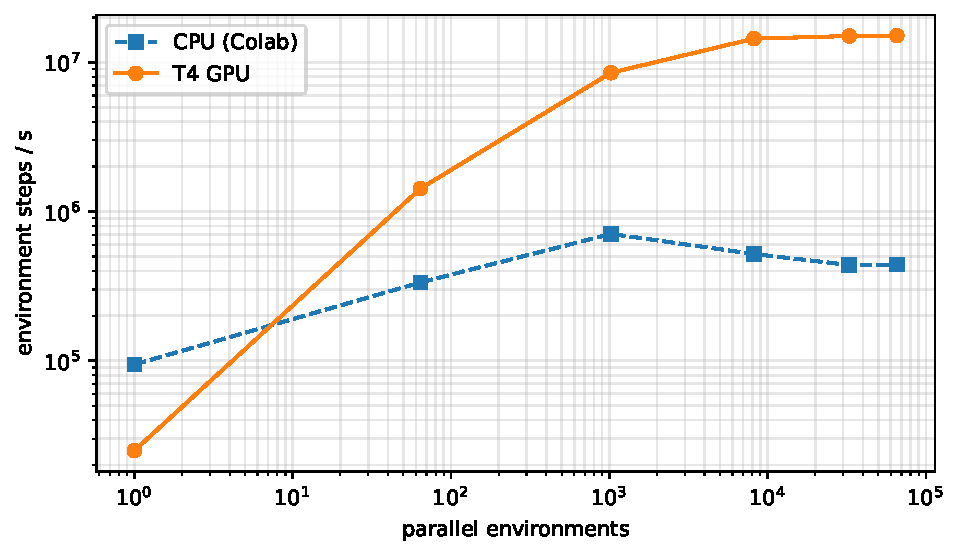
\includegraphics[keepaspectratio]{index_files/figure-pdf/fig-throughput-output-1.pdf}}

}

\caption{\label{fig-throughput}Drone environment throughput against the
number of parallel environments, one 500-step episode per environment.}

\end{figure}%

On the CPU, throughput peaks at 708k steps/s with 1,024 environments and
then falls as the batch outgrows the cache. On the T4 it keeps rising to
15.1M steps/s at 65,536 environments, 34× the CPU at the same size
(Figure~\ref{fig-throughput}). With a single environment the GPU is
slower than the CPU (25k vs 94k steps/s), because launch overhead
dominates. TPU numbers will appear here once
\texttt{notebooks/tpu\_run.ipynb} has been run.

\subsection{Drone}\label{drone}

With \(n=2048\), \(k=5\) (10,240 environments per generation) and 500
generations on the T4, the drone goes from a return of -4.1 (crashing,
no targets) to 77.0 with 9.2 targets per 10-second episode (average of
the last 10 generations: 75.1, 8.7 targets). The best generation was 468
(86.6). The whole run took 1.5 minutes. Most of the gain comes in the
first \textasciitilde40 generations; after that the return plateaus.

\subsection{The pendulum is solvable, but ES is
bimodal}\label{the-pendulum-is-solvable-but-es-is-bimodal}

The hand-written controller scores -139.5 ± 88.7 (median -121.9) over
100 episodes, well inside the solved range. The environment is therefore
not the cause of the −760 plateau.

\begin{longtable}[]{@{}
  >{\raggedright\arraybackslash}p{(\linewidth - 8\tabcolsep) * \real{0.1875}}
  >{\raggedright\arraybackslash}p{(\linewidth - 8\tabcolsep) * \real{0.1875}}
  >{\centering\arraybackslash}p{(\linewidth - 8\tabcolsep) * \real{0.2500}}
  >{\raggedleft\arraybackslash}p{(\linewidth - 8\tabcolsep) * \real{0.1875}}
  >{\raggedleft\arraybackslash}p{(\linewidth - 8\tabcolsep) * \real{0.1875}}@{}}

\caption{\label{tbl-seeds}Pendulum seed studies. Final return is the
trained mean policy on 100 fresh full-task episodes; solved means better
than −200.}

\tabularnewline

\toprule\noalign{}
\begin{minipage}[b]{\linewidth}\raggedright
Study
\end{minipage} & \begin{minipage}[b]{\linewidth}\raggedright
Device
\end{minipage} & \begin{minipage}[b]{\linewidth}\centering
Seeds solved
\end{minipage} & \begin{minipage}[b]{\linewidth}\raggedleft
Median final return
\end{minipage} & \begin{minipage}[b]{\linewidth}\raggedleft
Best final return
\end{minipage} \\
\midrule\noalign{}
\endhead
\bottomrule\noalign{}
\endlastfoot
small pop & CPU & 1 / 8 & -752.0 & -191.3 \\
curriculum & CPU & 0 / 8 & -759.7 & -207.8 \\

\end{longtable}

\begin{figure}[H]

\centering{

\pandocbounded{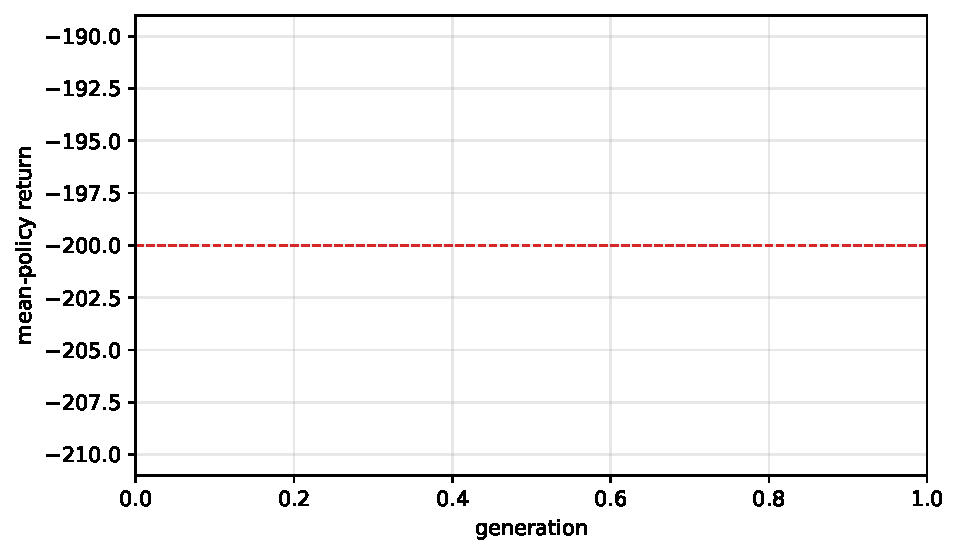
\includegraphics[keepaspectratio]{index_files/figure-pdf/fig-seeds-output-1.pdf}}

}

\caption{\label{fig-seeds}Mean-policy return per generation for every
seed of the CPU small-population study. Solved seeds in green, stuck
seeds in grey.}

\end{figure}%

With identical hyperparameters, 1 of 8 seeds solve the swing-up
(Table~\ref{tbl-seeds}, Figure~\ref{fig-seeds}). 2 of 8 leave the
plateau at all (1 of them narrowly misses the threshold, at -240). The
other 6 finish between -767 and -740: a policy that spins or hangs near
the bottom instead of balancing. The curriculum does not help: 0 of 8
seeds solved, median -760. Starting near upright teaches balancing, but
balancing does not lead to swinging up, so the hard part of the task is
still unsolved when the start range widens.

In exploratory runs we also varied \(\sigma\) (0.05--0.1, with and
without decay), the learning rate, the number of episodes per member
(4--16), the network width (32 or 64 units) and weight decay (0 or
0.005). None of these consistently removed the plateau. The same setting
solved the task from one seed and failed from another. Even changing how
often the training loop logs, which changes how the random-key stream is
split, flipped individual outcomes. Our earlier sweep trained every
configuration from the same single seed, so its ranking of
configurations mostly reflects which random streams happened to escape
the plateau.

\section{Discussion}\label{discussion}

\textbf{Speed is not the bottleneck; exploration is.} On a T4 a pendulum
run takes well under a minute, yet most runs end in the same local
optimum. For ES on this task, a run's outcome is a random variable and
should be reported as a success rate with its spread, as argued for deep
RL by Henderson et al. (2018).

\textbf{What would likely help.} The plateau is a known difficulty of
swing-up, which needs an energy-pumping phase before balancing (Åström
and Furuta 2000). Options we have not yet tested:

\begin{itemize}
\tightlist
\item
  \emph{Parallel restarts.} Run many independent ES instances, which is
  itself a \texttt{vmap}, and keep the best. At a success rate of \(p\)
  per seed, \(m\) restarts succeed with probability \(1-(1-p)^m\).
\item
  \emph{Larger or adaptive exploration}, for example novelty bonuses or
  a \(\sigma\) schedule driven by stagnation.
\item
  \emph{Better curricula}, such as reverse curricula that start from
  states the current policy can already reach (Florensa et al. 2017)
  instead of a fixed angle schedule (Bengio et al. 2009).
\item
  \emph{Simpler policies.} Linear policies with random search are
  competitive on many control tasks (Mania et al. 2018).
\end{itemize}

\textbf{Limitations.} Two small tasks; one policy architecture; the CPU
seed studies use 8 seeds each, so the success rates are coarse; the
drone was trained from a single seed. The TPU study (12 seeds per
setting, three settings) is defined in \texttt{colab\_run.py\ -\/-tpu}.
Its numbers appear in Table~\ref{tbl-seeds} and
Figure~\ref{fig-throughput} automatically once it has run.

\section{Reproducibility}\label{reproducibility}

All code is at \url{https://github.com/shiroonigami23-ui/jax-swarm-es}.
This paper is a Quarto document whose numbers, tables and figures are
computed from the files in \texttt{results/} each time it is rendered.
The commands are:

\begin{itemize}
\tightlist
\item
  \texttt{python\ -m\ swarm\_es.bench}: throughput.
\item
  \texttt{python\ -m\ swarm\_es.baselines}: the hand-written controller.
\item
  \texttt{python\ -m\ swarm\_es.seeds}: seed studies.
\item
  \texttt{notebooks/tpu\_run.ipynb}, which calls
  \texttt{colab\_run.py\ -\/-tpu}: the full TPU study.
\end{itemize}

\section*{References}\label{references}
\addcontentsline{toc}{section}{References}

\protect\phantomsection\label{refs}
\begin{CSLReferences}{1}{1}
\bibitem[\citeproctext]{ref-astrom2000}
Åström, Karl Johan, and Katsuhisa Furuta. 2000. {``Swinging up a
Pendulum by Energy Control.''} \emph{Automatica} 36 (2): 287--95.

\bibitem[\citeproctext]{ref-bengio2009curriculum}
Bengio, Yoshua, Jérôme Louradour, Ronan Collobert, and Jason Weston.
2009. {``Curriculum Learning.''} \emph{Proceedings of the 26th
International Conference on Machine Learning}, 41--48.

\bibitem[\citeproctext]{ref-jax2018}
Bradbury, James, Roy Frostig, Peter Hawkins, et al. 2018. \emph{{JAX}:
Composable Transformations of {Python+NumPy} Programs}. Released.
\url{http://github.com/jax-ml/jax}.

\bibitem[\citeproctext]{ref-brockman2016gym}
Brockman, Greg, Vicki Cheung, Ludwig Pettersson, et al. 2016.
{``{OpenAI} Gym.''} \emph{arXiv Preprint arXiv:1606.01540}.

\bibitem[\citeproctext]{ref-florensa2017reverse}
Florensa, Carlos, David Held, Markus Wulfmeier, Michael Zhang, and
Pieter Abbeel. 2017. {``Reverse Curriculum Generation for Reinforcement
Learning.''} \emph{Proceedings of the 1st Conference on Robot Learning}.

\bibitem[\citeproctext]{ref-freeman2021brax}
Freeman, C. Daniel, Erik Frey, Anton Raichuk, Sertan Girgin, Igor
Mordatch, and Olivier Bachem. 2021. {``Brax -- a Differentiable Physics
Engine for Large Scale Rigid Body Simulation.''} \emph{arXiv Preprint
arXiv:2106.13281}.

\bibitem[\citeproctext]{ref-henderson2018}
Henderson, Peter, Riashat Islam, Philip Bachman, Joelle Pineau, Doina
Precup, and David Meger. 2018. {``Deep Reinforcement Learning That
Matters.''} \emph{Proceedings of the AAAI Conference on Artificial
Intelligence}.

\bibitem[\citeproctext]{ref-kingma2015adam}
Kingma, Diederik P., and Jimmy Ba. 2015. {``Adam: A Method for
Stochastic Optimization.''} \emph{International Conference on Learning
Representations}.

\bibitem[\citeproctext]{ref-lange2022gymnax}
Lange, Robert Tjarko. 2022. \emph{Gymnax: A {JAX}-Based Reinforcement
Learning Environment Library}. Released.
\url{http://github.com/RobertTLange/gymnax}.

\bibitem[\citeproctext]{ref-lange2023evosax}
Lange, Robert Tjarko. 2023. {``Evosax: {JAX}-Based Evolution
Strategies.''} \emph{Proceedings of the Companion Conference on Genetic
and Evolutionary Computation}.

\bibitem[\citeproctext]{ref-mania2018}
Mania, Horia, Aurelia Guy, and Benjamin Recht. 2018. {``Simple Random
Search of Static Linear Policies Is Competitive for Reinforcement
Learning.''} \emph{Advances in Neural Information Processing Systems}.

\bibitem[\citeproctext]{ref-salimans2017}
Salimans, Tim, Jonathan Ho, Xi Chen, Szymon Sidor, and Ilya Sutskever.
2017. {``Evolution Strategies as a Scalable Alternative to Reinforcement
Learning.''} \emph{arXiv Preprint arXiv:1703.03864}.
\url{https://arxiv.org/abs/1703.03864}.

\bibitem[\citeproctext]{ref-uhlenbeck1930}
Uhlenbeck, George E., and Leonard S. Ornstein. 1930. {``On the Theory of
the Brownian Motion.''} \emph{Physical Review} 36 (5): 823--41.

\bibitem[\citeproctext]{ref-wierstra2014}
Wierstra, Daan, Tom Schaul, Tobias Glasmachers, Yi Sun, Jan Peters, and
Jürgen Schmidhuber. 2014. {``Natural Evolution Strategies.''}
\emph{Journal of Machine Learning Research} 15: 949--80.

\end{CSLReferences}




\end{document}
